\documentclass[tikz,border=18pt]{standalone}
\usetikzlibrary{patterns}

\pgfdeclarepatternformonly[\radius,\thickness,\size]{rings}
  {\pgfpoint{-0.5*\size}{-0.5*\size}}
  {\pgfpoint{ 0.5*\size}{ 0.5*\size}}
  {\pgfpoint{     \size}{     \size}}
  {\pgfsetlinewidth{\thickness}
   \pgfpathcircle\pgfpointorigin{\radius}
   \pgfusepath{stroke}}

\newdimen\thickness
\newdimen\radius

\tikzset{
  size/.store in=\size, size=9pt,
  thickness/.code={\pgfmathsetmacro\thickness{#1}},
  radius/.code={\pgfmathsetmacro\radius{#1}},
  outer/.style={thickness=2*\size*(sqrt(3)-1)/(2*sqrt(6)),
                   radius=  \size*(sqrt(3)+1)/(2*sqrt(6))},
  mezzo/.style={thickness=2*\size*(sqrt(2)-1)/(2*sqrt(3)),
                   radius=  \size*(sqrt(2)+1)/(4*sqrt(3))},
  inner/.style={thickness=  \size/(2*sqrt(3)),
                   radius=  \size/(4*sqrt(3))},}

\begin{document}
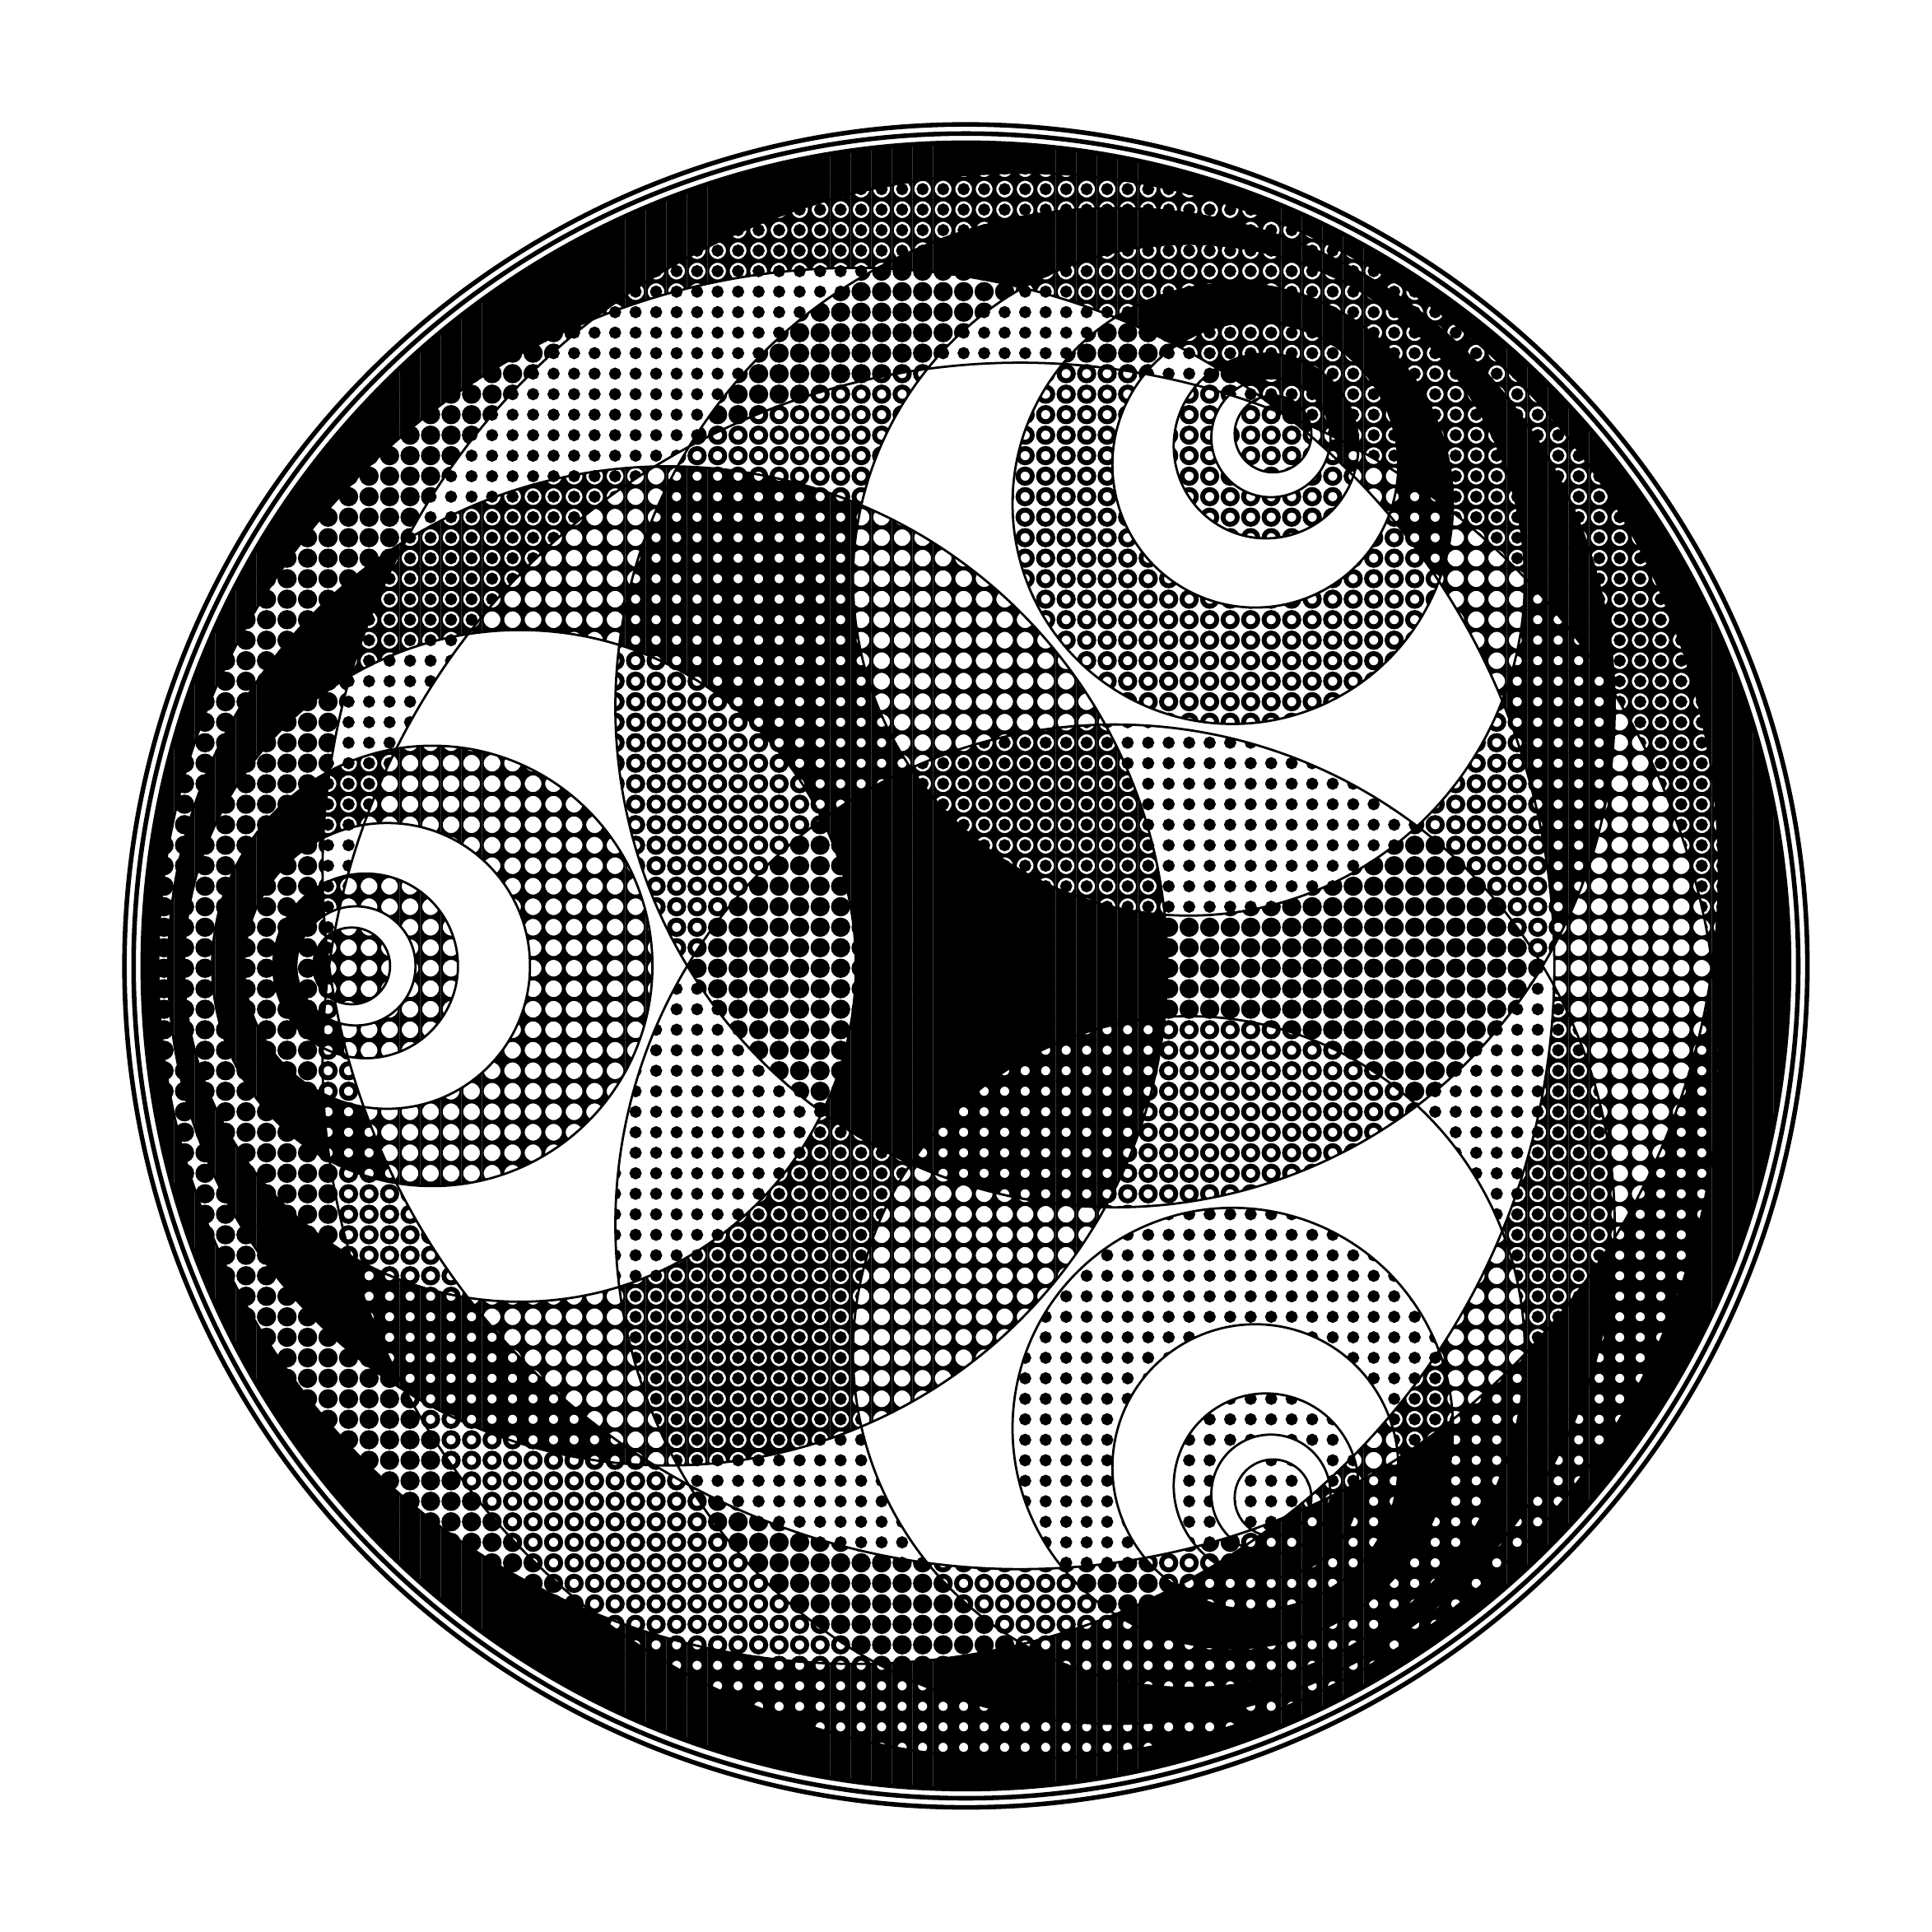
\begin{tikzpicture}

\foreach \r/\style in {180/outer,60/mezzo,-60/inner}{
  \begin{scope} [rotate=\r]
    \filldraw [line width=1bp, even odd rule, pattern=rings, \style]
      \foreach \n in {1,0.9,...,0.1}{
        ({5*54bp*(1-sin(90*exp(ln(9)*(\n))/9)^4)},0)
        circle ({5*72bp*sin(90*(exp(ln(81)*\n)/81))})};
  \end{scope}}

\draw [line width=2bp]
  \foreach \n in {0,2,4}{
    circle ({5*72bp+\n*\pgflinewidth}) };

\end{tikzpicture}
\end{document}
